\documentclass[12pt]{article}

\usepackage{tgtermes}
\usepackage{epsf}
\usepackage{epstopdf}
\usepackage{amsmath}
\usepackage{graphicx}
\usepackage{booktabs}
\usepackage[colorlinks=true,linkcolor=blue,citecolor=blue]{hyperref}
\usepackage{dcolumn}
\usepackage{amsmath, amsthm, amssymb}
\usepackage{mwe}
\usepackage{url}
%\usepackage{harvard}
\usepackage{fancyheadings}
\usepackage{longtable}
\usepackage{authblk}
\usepackage{setspace}
%\usepackage[nomarkers]{endfloat}
\usepackage{float}
\usepackage{bbm}
%\usepackage{titling}
\usepackage{subcaption}
\usepackage{algorithm}
\usepackage{algorithmic}
\usepackage{import}
\usepackage[backend=biber,style=authoryear,
sorting=ynt,citestyle=authoryear]{biblatex}
\addbibresource{papercitations.bib}
%\usepackage[nomarkers,nofiglist,notablist]{endfloat}
\usepackage{subcaption}
\usepackage{caption}

\onehalfspacing
\textwidth 6.5in \oddsidemargin 0in \evensidemargin -0.6in
\textheight 8.5in \topmargin -0.2in

\newcolumntype{L}[1]{>{\raggedright\let\newline\\
		\arraybackslash\hspace{0pt}}m{#1}}
\newcolumntype{C}[1]{>{\centering\let\newline\\
		\arraybackslash\hspace{0pt}}m{#1}}
\newcolumntype{R}[1]{>{\raggedleft\let\newline\\
		\arraybackslash\hspace{0pt}}m{#1}}
\newcolumntype{P}[1]{>{\raggedright\tabularxbackslash}p{#1}}

\newtheorem{theorem}{Theorem}[section]
\newtheorem{corollary}[theorem]{Corollary}
\newtheorem{proposition}[theorem]{Proposition}
\newtheorem{lemma}[theorem]{Lemma}

\captionsetup{justification=centering,singlelinecheck=false}


\newcommand{\xsub}[1]{%
	\mbox{\scriptsize\begin{tabular}{@{}c@{}}#1\end{tabular}}%
}

%\renewcommand{\thetable}{\Roman{table}}

\begin{document}
	
	
	
	
	\linespread{1.2}\title{\vspace{-0.5in} Overlapping Board Members in the Hospital Industry} 
	
	\date{\today}
	
	\author{\vspace{10mm}Hanna Glenn\footnote{Department of Economics, Emory University, 1602 Fishburne Drive, Atlanta, GA 30322, hanna.glenn@emory.edu.} }
	
	\maketitle
	%\setlength{\droptitle}{-10pt}
	
	\vspace{-0.2in}
	
	\singlespacing\maketitle


 \vspace{3mm}
	
    \begin{abstract}
		{\small
    Consolidation in health care has been a heavily discussed topic in research and regulation, as more concentration has been linked to higher prices and lower quality. Aside from formal mergers and acquisitions, there is opportunity for hospitals to form affiliations with other competing hospitals through sharing common board members, which has mainly been studied in the context of large public firms. This paper establishes the existence of overlapping board members in competing nonprofit hospitals in the US. Using a data set constructed from IRS Tax Form 990s, I show that 8\% of nonprofit hospitals have overlapping board members with an otherwise unaffiliated hospital, and 17\% of hospital referral regions have overlapping boards within the market. These findings highlight an understudied mechanism through which hospitals form affiliations, potentially affecting patient and market outcomes. 
		} 
	\end{abstract}
	
	
	
	
	

	
	\onehalfspacing
	
	\newpage

    \section{Introduction}

    Consolidation in health care remains a forefront concern for regulators in the US, as both horizontal and vertical integration have substantially increased over the last several decades (\cite{levinson2024ten}). Researchers have documented higher prices (\cite{brot2024pays}), and mixed effects on quality (\cite{kessler2000hospital}; \cite{cooper2011does}) as a result of health care becoming more concentrated through mergers and acquisitions. There is significant antitrust scrutiny in this sector, and proposed mergers are regularly denied due to expected harmful effects to competition (\cite{Meyer2022}). Firms in other industries have been shown to engage in methods of informal affiliation besides formal mergers and acquisitions. For example, instances of board overlap in public firms have been cited to violate the Clayton Act due to their anti-competitive nature. Yet, despite concerns of low competition, this type of connectedness among firms has not been given much consideration in health care. In this paper, I document the extent of overlapping board members in nonprofit hospitals in the US, and explore avenues of future research to investigate 
    potential anti-competitive effects of this type of affiliation.

    The presence of overlapping board members across firms, also referred to as board interlock, has been heavily studied in corporate finance, particularly for large publicly traded firms. By the Clayton Act of 1914, board overlap among sufficiently large competing firms is illegal. Yet, it is known to exist even among the largest publicly traded firms. Researchers have found that board overlap is correlated with governance practices, performance, investment in research and development, and product differentiation (\cite{cai2014board}; \cite{lamb2016ties}; \cite{geng2021does}). While the Department of Justice has increased scrutiny of board overlap, their focus has remained on tech and private firms (\cite{Morse2023}). Board overlap does occur in health care with instances of organizations denied merger permission due to boards not acting independently (\cite{huberfeld2006tackling}), of hospitals declaring informal affiliations through leadership (\cite{barnett_babcock_2012}), and of life sciences companies with substantial documented overlap (\cite{manjunath2024illegal}). However, little is known about how prevalent board overlap is in the hospital industry, and whether it is correlated with other hospital characteristics. 

    In this paper, I form networks of hospital board of director members using Tax Form 990s, which requires nonprofits in the US to declare the identities and compensation information of their board. Extracting these identities and matching to other sources of hospital information, I show that approximately 8\% of the nonprofit hospitals in the sample are affiliated with another hospital in the same market through shared board members, even excluding system or network affiliations. Among hospitals that share board members, two thirds of the hospital pairs are between two general adult hospitals. That is, a majority of the shared board members serve on directly competing hospitals in the same geographic market. 

    Establishing descriptive evidence of board overlap in hospitals, this paper encourages future research to take seriously this behavior as potentially having downstream effects for patients. While formal integration in health care should not be overlooked, there is a call for future research to scrutinize other forms of firm allegiance in policy and regulation. 


    \section{Related Literature}\label{sec:relatedlit}


    \subsection{Overlapping Board Members}\label{sec:boardoverlaplit}

    One of the first studies of board overlap argues that firms are not independent, self-sufficient organisms in the economy, but are actually heavily interconnected via overlapping board members (\cite{dooley1969interlocking}). Dooley frames board interlock as ``the root of many evils", and finds several aspects of corporations to be correlated with whether they share board members with another corporation: size, financial relationships with other companies, and management control. This paper led to a number of studies focusing on how board interlock affects corporate governance, including whether board overlap stretches individual board members too thin (\cite{ferris2003too}; \cite{field2013busy}), contributes to increases in backdating stock options (\cite{bizjak2009option}), or led to convergence in governance strategy and behavior (\cite{bouwman2011corporate}; \cite{chiu2013board}; \cite{cai2014board}). 

    The literature thus establishes a strong link between board interlock and governance practices. However, the relationship between board overlap and firm behavior, particularly its impact on competition, remains less understood. Theoretically, the direction of this effect is ambiguous. On one hand, board interlock is often viewed as an anti-competitive practice that enables implicit collusion. Alternatively, firms may seek highly experienced and connected individuals for their boards, leading to valuable knowledge sharing and enhanced decision-making. Most studies in this area have focused on the financial performance implications of board overlap, with firm behavior considered primarily as a mediating mechanism.

    Two main studies analyze of the effect of board overlap on financial performance. First, \citeauthor{baran2017director} (\citeyear{baran2017director}) leverages entry and exit from the S\&P 500, along with variation in the local supply of directors, and finds that well-connected board members contribute positively to firm value. Similarly, leveraging policies in the US that remove barriers to board overlap, \citeauthor{geng2021does} (\citeyear{geng2021does}) finds that board overlap leads to higher profitability. 
    
    Beyond financial performance, several studies explore the relationship between board overlap and firm investment decisions, including mergers and acquisitions, research and development (R\&D), and technology investment. \citeauthor{schonlau2009board} (\citeyear{schonlau2009board}) and \citeauthor{cai2012board} (\citeyear{cai2012board}) analyze financial performance after mergers and acquisitions of publicly traded firms with connected boards, finding that firms with board overlap are more likely to be involved in acquisitions, and that specific types of board connections lead to better financial performance for the acquirer after the transaction. One paper examines whether interconnected firms are more likely to invest in the same information technology, and finds a positive association between board overlap and investment in IT among firms with active boards, indicating that timely communication is an important factor in whether board overlap matters (\cite{cheng2021social}). Finally, \citeauthor{geng2021does} (\citeyear{geng2021does}) finds that lower research and development expenditure and more product differentiation are key mechanisms through which overlapping firms improve profitability. 

    Despite these insights, significant gaps remain in our understanding of board overlap. Research has largely focused on governance or firm-level performance, while firm behavior and the broader market implications of board overlap remain underexplored. Additionally, most studies have been limited to large, publicly traded firms. This focus stems from the assumption that nonprofits engage in less anti-competitive behavior (\cite{baer2014clayton}; \cite{aai2013section7}), making board overlap in such organizations less concerning. However, this assumption is flawed, particularly in industries like health care, where nonprofit hospitals dominate and have been shown to engage in anti-competitive practices (\cite{hulver2023ftc}). Further research is needed to assess the competitive effects of board overlap across different market settings, particularly in nonprofit sectors where such dynamics may have substantial implications for industry competition and consumer welfare. I draw from this literature to inform potential outcomes of interest when considering board overlap in hospitals: financial performance, mergers and acquisitions, investment, and product differentiation. I discuss in Section \ref{sec:hospbehaviors} how these outcomes related to hospitals specifically. 





    \subsection{Common Ownership}\label{sec:commonownerlit}

    As consolidation in investment companies and in many industries has increased over time, so has the prevalence of common ownership among publicly traded firms. That is, firms within the same industry and market are increasingly owned by the same investment companies. While a separate occurrence and literature than that of board overlap, there are numerous parallels between the two concepts. Unlike publicly traded firms, nonprofits do not have shareholders that receive dividend payments. However, in some ways, a board functions similarly to shareholders: they influence the strategic direction of the organization through information sharing and voting on firm decisions without actively managing day-to-day operations. Further, the literature on common ownership in relation to market concentration and economic incentives is more developed than that of board overlap. Thus, I draw on this literature to inform outcomes that are potentially related to board overlap in the hospital industry. 
    
    Whether common ownership affects competition is a widely debated theme in the economics literature. Theoretical models predict that common ownership will lead to lower equilibrium output and higher markups through firms placing non-zero weight on competitors' profit (\cite{rubinstein1983competitive}; \cite{rotemberg1984financial}; \cite{azar2012new}). Empirical evidence has grown tremendously since the seminal studies by \citeauthor{he2017product} (\citeyear{he2017product}) and \citeauthor{azar2018anticompetitive} (\citeyear{azar2018anticompetitive}), who found that common ownership leads to greater consolidation (acquisitions, joint ventures, strategic alliances), and that common ownership led to higher prices in the airline industry, respectively. However, these findings have been critiqued for how they measure common ownership and endogeneity concerns (\cite{kennedy2017competitive}; \cite{lewellen2021does}).

    A number of studies have since attempted to estimate the effect of common ownership on a range of outcomes including prices, research and development, merger activity, and patent durability (\cite{gerardi2023critical}). Many of which document a statistically significant relationship between common ownership and the relevant outcome. However, recent studies using alternative identification strategies find that common ownership can actually increase competition through lower insider trading profits, more product development, and higher investments (\cite{chen2023does}; \cite{kini2024common}). Additionally, recent literature has considered common ownership in the context of private firms with venture capitalists, where consolidated ownership is even more prevalent, and has found that competition decreases and information sharing increases in this setting (\cite{lindsey2008blurring}; \cite{gonzalez2020exchanges}; \cite{li2023common}; \cite{eldar2024common}).

    The literature on common ownership yields several conclusions for a study on board overlap. The first is a theoretical foundation confirming the importance of particular outcomes relevant to competition and consumer welfare, including merger and acquisition activity and investment decisions. Second, the common ownership literature focuses much more on how prices are impacted, which is also relevant in the health care setting. Finally, this literature introduces important concerns about the endogenous choice of owners or board members. While this study does not seek to causally estimate the effects of board overlap in hospitals, this is an important consideration for future research. 
    

    \subsection{Consolidation in Hospitals}

    There is a rich empirical literature examining the effects of consolidation in health care that includes both vertical and horizontal integration between hospitals, practices, and physicians. As the focus of this paper is affiliation among competing hospitals, I draw on the literature examining hospital consolidation through mergers and systems to inform hospital behaviors that might be correlated with board overlap but are unique to the hospital setting and thus weren't discussed in Section \ref{sec:boardoverlaplit}. The main outcomes of interest in this area of research have centered around price and quality of care. 

    Early studies on hospital consolidation found very little evidence of impacts on operating costs, efficiency, or quality of care (\cite{alexander1996short}; \cite{ho2000hospital}; \cite{dranove2003hospital}). From 2000-2020, the occurrence of hospital mergers increased dramatically, where a quarter of hospital markets included zero independent hospitals by 2020 (\cite{ElevanceHealth2023}). This increased concentration has led to a vast number of studies estimating its effect on quality, operating costs, and prices. 

    Studies typically document cost and efficiency gains experienced by hospitals who merge to become part of a larger system (\cite{schmitt2017hospital}; \cite{andreyeva2024corporatization}), even if the effects are small (\cite{craig2021mergers}). Naturally, this leads to the question of whether such efficiency gains are passed through to patients by lower prices. Across various settings, data sources, and methodology, hospital mergers are associated with significant increases in price due to hospitals having greater negotiating power with insurance companies (\cite{gaynor2012impact}; \cite{boozary2019association}; \cite{cooper2019price}; \cite{andreyeva2024corporatization}). 
    
    There is mixed evidence on whether such gains in efficiency translate to better quality of care.  Several studies comparing hospitals who became a part of a system with observably similar hospitals that did not merge find little to no effect on readmission or mortality rates on average (\cite{haas2011mergers}; \cite{beaulieu2020changes}). However, one study finds that among heart disease patients, treatment intensity and mortality rates both increase after hospital consolidation (\cite{hayford2012impact}), and another finds increased readmission rates across all types of patients (\cite{andreyeva2024corporatization}). 

    A select number of studies investigate other dimensions that could be affected by more system affiliation over time. In a slightly different setting of acquisitions of dialysis centers, \citeauthor{eliason2020acquisitions} (\citeyear{eliason2020acquisitions}) finds that decreases in quality are driven primarily by the convergence of treatment styles among acquired centers and their acquirer. Additional studies have suggested that consolidated service offerings is a potential mechanism for effects on quality (\cite{mariani2022impact}). Finally, \citeauthor{desai2023hospital} (\citeyear{desai2023hospital}) examine admission patterns of low-income patients as a result of increased hospital concentration, and find that Medicaid admissions decrease as a result of increased concentration. That is, highly concentrated markets redistribute patients within the market (\cite{desai2023hospital}). 

    This literature informs ways that hospital affiliations could affect firm behaviors and outcomes specific to hospitals. In addition to the behaviors discussed in Sections \ref{sec:boardoverlaplit} and \ref{sec:commonownerlit}, measures of quality of care, treatment styles, service offerings, and admission patterns could also be important aspects driven by affiliation with other hospitals. I discuss these in more detail in Section \ref{sec:hospbehaviors}. 

    

    \subsection{Informing Hospital Behaviors}\label{sec:hospbehaviors}

    The main purpose of this paper is to document the prevalence of board overlap in US hospitals in Section \ref{sec:document}. While I do not establish any causal relationship between board overlap and hospital behaviors, I consider the literature on board overlap, common ownership, and hospital consolidation discussed in Section \ref{sec:relatedlit} to inform a set of hospital behaviors that may be relevant for future research. I divide these behaviors into three categories: price/quality, investment decisions, and differentiation. 

    The hospital consolidation literature highlights price and quality of care as key factors in the industry. Mergers often grant hospitals greater market power, enabling them to negotiate higher prices with insurance companies. It is unclear whether shared board members would lead to similar price increases. If board overlap facilitates information sharing about negotiations, it could indirectly influence pricing. However, direct board involvement in pricing decisions seems less likely. Nevertheless, with access to data on actual prices charged by hospitals, this remains an interesting outcome for future research to explore.

    It seems more likely that quality of care could be impacted by overlapping board members among hospitals. There are direct actions that could lead to changes in quality such as convergence in treatment styles or investment in technology, which I will discuss in detail in the following sections. There is also an indirect path through which overlapping board members might impact quality, which is that hospitals might compete for the same pool of experienced board members. If the board members with the most expertise are in high demand, sharing that expertise among multiple hospitals could facilitate greater improvements. The most commonly used measurements of quality of care in hospitals are mortality and readmission rates. 

    In both board overlap and common ownership, several investment decisions are shown to be associated with established firm affiliation. First, hospitals with board shared board members might be more likely to merge in the future. Second, sharing board members could facilitate engaging in the same types of technology or capital. Therefore, an area of future research is to look at outcomes such as health information technology investments, specific medical technology advancements in the hospital, and capital investments. 

    Finally, previous research has shown that product differentiation is associated with board overlap in other industries. That is, sharing information among competing hospitals can lead to more specialization. In hospitals, there are two distinct types of differentiation: either through services offered, or the types of patients admitted. Both of these behaviors are key findings in the hospital merger literature, indicating that affiliations through board members could also facilitate changes in these areas. In future research, one could think about measuring the likelihood of specialized services being offered, such as a Neonatal Intensive Care Unit or cardiac catheterization laboratory, where hospitals might shift investments towards services not offered by their affiliated hospital. Additionally, patient composition in the hospital, measured by the payer mix of admitted patients or complexity of their conditions, could be compared among hospitals with and without shared board members. 

    


    

    \section{Documenting Overlapping Board Members in US Hospitals}\label{sec:document}

    \subsection{Data Construction}

    
   I compile data on nonprofit hospital board of directors from publicly available Tax Form 990s, which all sufficiently large nonprofits must file with the Internal Revenue Service (IRS) each year. These forms contain a section in which nonprofits declare their board, executives, and highest compensated employees. This paper focuses only on the board of director identities. I limit to firms that fill out Schedule H of the tax form, an indicator that the firm operates a hospital. PDF versions of the 990s are made publicly available by Nonprofit Explorer dating back at least 20 years. However, using optical character recognition text extraction methods on these PDFs is both time consuming and can lead to small errors in names extracted. Since I rely heavily on the accuracy of matching individuals, I analyze the data from 2017 onward, when the IRS began publishing XML versions of these files, which ensures accurate names that can be matched across hospitals and time. This also provides a more current picture of the prevalence of board overlap in this industry. I extract all names and positions of individuals listed in the section titled ``Officers, Directors, Trustees, Key Employees, and Five Highest Compensated Employees". I also record information on the hospital that filed the tax form: the Employee Identification Number (EIN), organization name and location, and other characteristics. There are 2,096 hospitals in the initial extraction of firms and identities.

   Next, I match hospitals in the tax form data to hospitals in other publicly available data sources. The only common information about hospitals across these sources is the name and location. Therefore, I use fuzzy string matching methods to create a crosswalk of EINs to identification numbers in the American Hospital Association (AHA) survey data. Specifically, I compute the Jaro-Winkler distance between hospital names in each data set. Then, I record matches with sufficiently similar names and addresses. I have a sample of 1,623 hospitals in the tax data that can be linked to the AHA survey. 

    I limit the individuals in the sample to those on the board of directors, excluding executives that also serve on the board. I clean the board member names by removing common titles (Dr., Reverand, etc.), and combining names within the same firm that have slight spelling differences. For example, if John Matthews is a board member of hospital A in 2017, and John Matthew is a board member of hospital A in 2018, I assume these names represent the same person. Finally, to avoid issues in whether first or last names are listed first, I sort each individual's names alphabetically. 

    I define a hospital as having an overlapping board member if any of the individuals on their board are also on the board of a hospital in the same hospital referral region (HRR). HRRs are market designations created by Dartmouth Atlas using patient referral data which are meant to capture geographic regions of the average patient's choice set of health care facilities. I make this restriction first because board overlap is predicted to matter among competing firms, and hospitals compete for patients within the same geographic region. Additionally, hospital mergers have been shown to have a more significant effect when the entities involved are located geographically close (\cite{cooper2019price}). Therefore, the relevant measure for board overlap in hospitals should be those within the same market. 

    Another restriction that I place for two hospitals to share overlapping board members is that they must not be affiliated by system or network. It is common for within-system hospitals to either share common board members or be governed by the same over-arching board. However, systems are already formally affiliated, and this affiliation can dictate many of the behaviors I discuss in Section \ref{sec:hospbehaviors}. Therefore, I rely on variation in board overlap that does not include system affiliation. Therefore, any hospitals with board overlap in my sample are otherwise unaffiliated. There still may exist board overlap across systems. That is, I still consider hospital A belonging to System 1 as eligible to share board members with hospital B in System 2. 


    \subsection{Summary Statistics}

    First, I present a summary statistics table showing characteristics of all hospitals in the final sample, which consists of 1,466 nonprofit hospitals, almost all of which are adult general hospitals. They have, on average, 178 beds and 14 board members. Almost 40\% of the hospitals in the sample are academic medical centers, almost 70\% of the sample are located in metropolitan areas, and 56\% belong to a system. 

    \import{Objects}{all_summarystats.tex}

    Eight percent of hospitals in the sample have overlapping board members with an otherwise unaffiliated hospital. In Figure \ref{fig:connected_percent}, I show that this percentage remains relatively constant over time, with a slight decrease from 129 affiliated hospitals in 2017 to 114 affiliated hospitals in 2021. I include 2022 values, but there are less total firms in the sample due to lag in tax forms being made available publicly. As mentioned previously, common board members should be more likely to affect behavior within a hospital market, where hospitals compete for the same patient population. Therefore, in Figure \ref{fig:connected_HRR_percent}, I show the prevalence of having shared board members within a hospital market. Of the 306 HRRs in the US, approximately 17\% have at least one pair of board affiliated hospitals within the market. This proportion decreases slightly over time, with 15\% of HRRs having connected hospitals in 2021, a nominal decrease of 8 markets losing hospitals with affiliation. This is likely due to increased system affiliations, which mechanically decreases board overlap according to the definition I use here. 


    \begin{figure}[ht!]
        \centering
        \vspace{9mm}
        \caption{Percent of hospitals that have a board affiliation}
        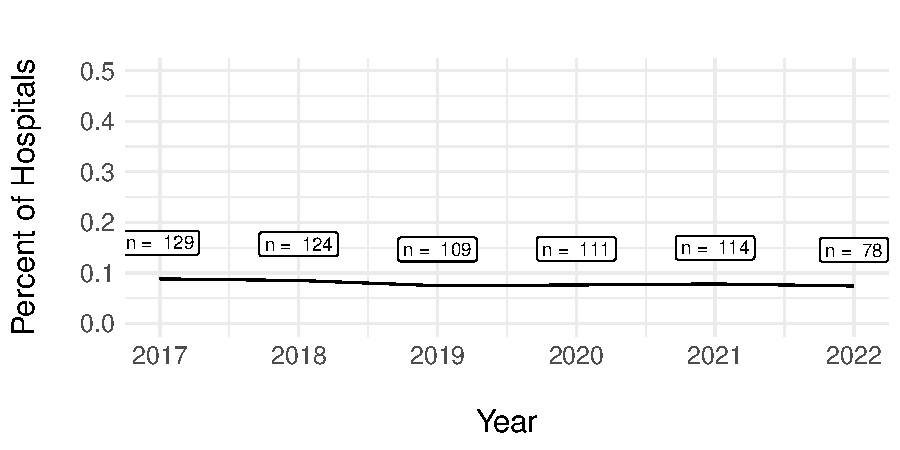
\includegraphics[width=.8\textwidth]{Objects/connected_percent.pdf}
        \label{fig:connected_percent}
    \end{figure}


    \begin{figure}[ht!]
        \centering
        \caption{Percent of HRRs containing board affiliated hospitals}
        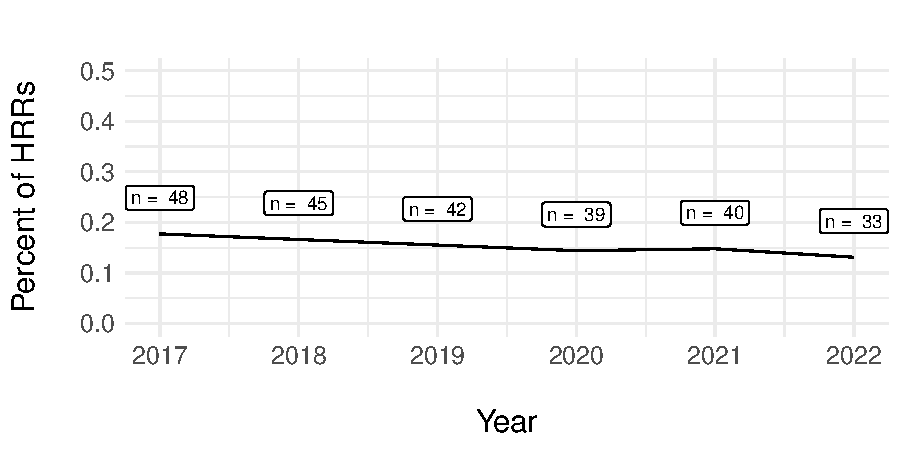
\includegraphics[width=.8\textwidth]{Objects/connected_HRR_percent.pdf}
        \label{fig:connected_HRR_percent}
    \end{figure}

    Next, I present geographic distribution of these pairs in Figure \ref{fig:connected_maps}. The blue lines represent hospitals that share a common board member, and the red dots are all other hospitals. Connected hospitals are distributed fairly evenly across the US, apart from relatively few connections on the west coast relative to the population. Over time, the connections remain fairly consistent geographically. Taken together, these show that board overlap is a prevalent occurrence among nonprofit hospitals in the US from 2017 onward. 

    \begin{figure}[ht!]
        \centering
        \caption{Geographic distribution of board affiliated hospitals over time}
        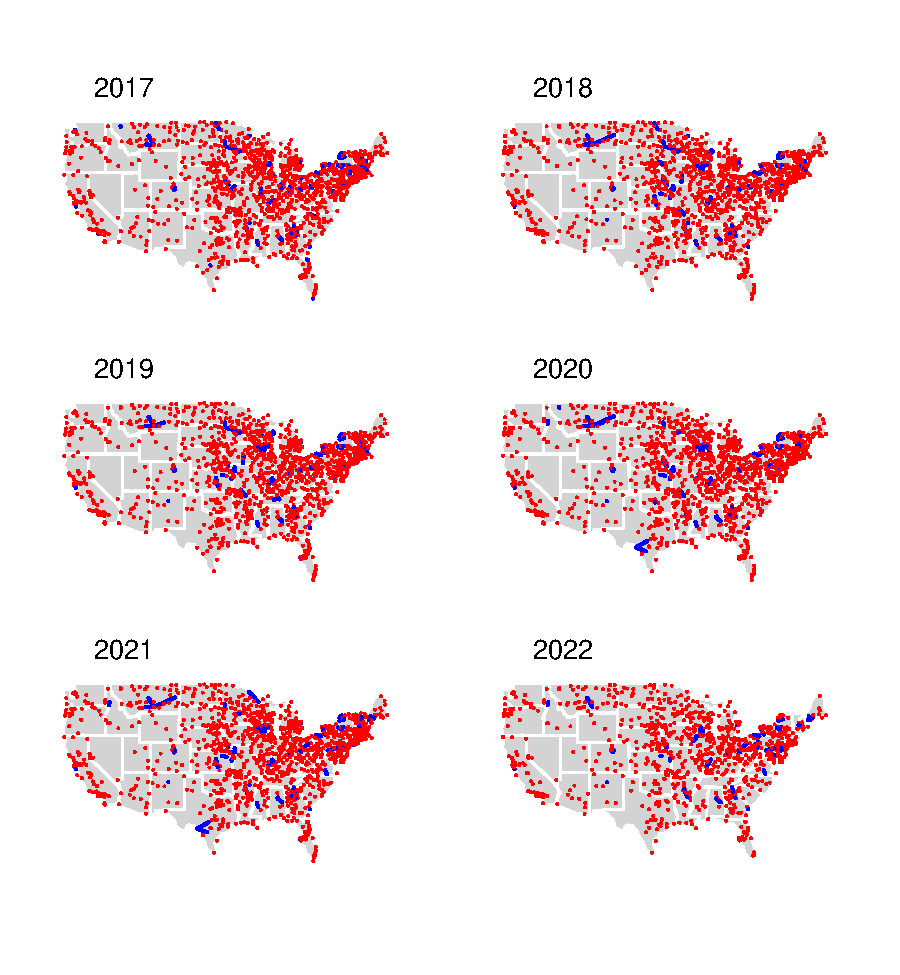
\includegraphics[width=\textwidth]{Objects/connected_maps.pdf}
        \label{fig:connected_maps}
    \end{figure}



    I now shift to examining characteristics of hospitals with board overlap. I present the proportion of the type of hospital pairs in Table \ref{tab:hospital_pair_types}. Each hospital is general or specialty (I only consider adult hospitals for these categories), children or adult, and independent or belonging to a system, all characteristics in the AHA data. Two-thirds of board affiliated pairs are between two adult general hospitals, and 10\% of pairs are between a specialty and a general hospital. Thus, for the majority of hospitals that have board interlock, the hospital they share a board member with is a direct competitor. 

    \import{Objects}{hospital_pair_types.tex}
    
    There is also significant variation in the ownership type of hospitals within affiliated pairs. Forty-five percent of pairs are between two non-system affiliated hospitals, and 36\% of pairs are between an independent hospital affiliated with a hospital belonging to a system. The lowest proportion of shared board member pairs is made up of two hospitals belonging to different systems. In total, there are 217 hospitals that share a board member with at least one other hospital at some point in the sample. 

    Considering general hospitals with shared board members, how different are


    I now shift towards examining summary statistics of hospitals with different types of affiliation relationships. First, in Table \ref{tab:hospital_general_summarystats}, I focus on general hospitals in four categories: board affiliated with another general hospital, board affiliated with a specialty hospital, unaffiliated through board members but belonging to a system, and completely unaffiliated. I present means of hospitals in each of these categories for the number of beds, the number of patients seen, whether it is an academic medical center, whether the hospital is located in a metropolitan area, and whether the hospital belongs to a system. On these dimensions, hospitals affiliated with other general hospitals (column 1) are relatively similar to unaffiliated hospitals that are part of a system (column 3). Unaffiliated hospitals that are not part of a system are slightly smaller in terms of bed size and number of patients seen, and less likely to be in a metropolitan area. The hospitals in column (2) are outliers, with a large number of beds and patients seen, and mainly in metropolitan areas. There are only 12 hospitals in this sample that are likely very different from the average general hospital. 

    \import{Objects}{hospital_general_summarystats.tex}

    I also present means of various measures of patient demographics, include the number of Medicare and Medicaid patients normalized by total beds, the total number of Medicare patients from CMS, the average Medicare patient age, and the average Medicare patient risk score. These measures yield similar descriptive results, that the unaffiliated hospitals that are not part of a system are slightly smaller, but they see similar patients in terms of age and complexity. Finally, I show means of variables to capture aspects of the service offerings of the different types of hospitals. First, from the AHA survey, I include an indicator for whether the hospital offers services in a Neonatal Intensive Care Unit (NICU) or Cardiac catheterization lab, both specialized and profitable services. General hospitals that are affiliated with specialty hospitals are the most likely to offer these services. Hospitals without any board member affiliations but belonging to a system are more likely to offer these services than unaffiliated hospitals that do not belong to a system. Hospitals that are affiliated with another general hospitals fall somewhere in between these two, with slightly less likelihood than the unaffiliated hospitals belonging to a system. I also include a measure of the concentration of bed allocation, where a higher concentration indicates that a hospital's bed capacity is concentrated in fewer service categories, whereas a lower concentration suggests a more diversified service offering. I also compute a similar concentration metric using the percent of patients in several service categories from the CMS Provider Utilization Files. For both measures, there seems to be little variation in service concentration across affiliation types.

    Next, I present the same summary statistics for specialty hospitals with different types of affiliations: affiliated with a general hospital, unaffiliated through board but belonging to a system, and unaffiliated through board or system, shown in Table \ref{tab:hospital_specialty_summarystats}. Overall, there are less specialty hospitals included in the sample, and very few of them are affiliated through board members. Specialty hospitals are more concentrated than general hospitals, as expected. In the AHA measure of concentration, all specialty hospitals are similarly concentrated. However, when using the services included in the CMS files, the concentration of unaffiliated system hospitals is much lower than that of any other specialty hospital. This could be due to the limited services included in the CMS data. Since this is such a small and specialized sample of hospitals, I do not include them in the main analysis. 

    \import{Objects}{hospital_specialty_summarystats.tex}
    
    


  

    \newpage


    \printbibliography


    

    

    

    

    

	
	
	


\end{document}